\documentclass{article} % For LaTeX2e
\usepackage{nips14submit_e,times}
\usepackage{amsmath}
\usepackage{amsthm}
\usepackage{amssymb}
\usepackage{mathtools}
\usepackage{hyperref}
\usepackage{url}
\usepackage{algorithm}
\usepackage[noend]{algpseudocode}
%\documentstyle[nips14submit_09,times,art10]{article} % For LaTeX 2.09

\usepackage{mathrsfs}
\usepackage{graphicx}
\usepackage{caption}
\usepackage{subcaption}

\def\eQb#1\eQe{\begin{eqnarray*}#1\end{eqnarray*}}
\def\eQnb#1\eQne{\begin{eqnarray}#1\end{eqnarray}}
\providecommand{\e}[1]{\ensuremath{\times 10^{#1}}}
\providecommand{\pb}[0]{\pagebreak}

\newcommand{\E}{\mathrm{E}}
\newcommand{\Var}{\mathrm{Var}}
\newcommand{\Cov}{\mathrm{Cov}}

\def\Qb#1\Qe{\begin{question}#1\end{question}}
\def\Sb#1\Se{\begin{solution}#1\end{solution}}

\newenvironment{claim}[1]{\par\noindent\underline{Claim:}\space#1}{}
\newtheoremstyle{quest}{\topsep}{\topsep}{}{}{\bfseries}{}{ }{\thmname{#1}\thmnote{ #3}.}
\theoremstyle{quest}
\newtheorem*{definition}{Definition}
\newtheorem*{theorem}{Theorem}
\newtheorem*{lemma}{Lemma}
\newtheorem*{question}{Question}
\newtheorem*{preposition}{Preposition}
\newtheorem*{exercise}{Exercise}
\newtheorem*{challengeproblem}{Challenge Problem}
\newtheorem*{solution}{Solution}
\newtheorem*{remark}{Remark}
\usepackage{verbatimbox}
\usepackage{listings}
\title{Linear Algebra II: \\
Problem Set IV}


\author{
Youngduck Choi \\
CIMS \\
New York University\\
\texttt{yc1104@nyu.edu} \\
}


% The \author macro works with any number of authors. There are two commands
% used to separate the names and addresses of multiple authors: \And and \AND.
%
% Using \And between authors leaves it to \LaTeX{} to determine where to break
% the lines. Using \AND forces a linebreak at that point. So, if \LaTeX{}
% puts 3 of 4 authors names on the first line, and the last on the second
% line, try using \AND instead of \And before the third author name.

\newcommand{\fix}{\marginpar{FIX}}
\newcommand{\new}{\marginpar{NEW}}

\nipsfinalcopy % Uncomment for camera-ready version

\begin{document}


\maketitle

\begin{abstract}
This work contains solutions to the problem set IV
of Linear Algebra II 2016 at Courant Institute of Mathematical Sciences.
\end{abstract}

\bigskip

\begin{question}[1]
\hfill
\begin{figure}[h!]
  \centering
    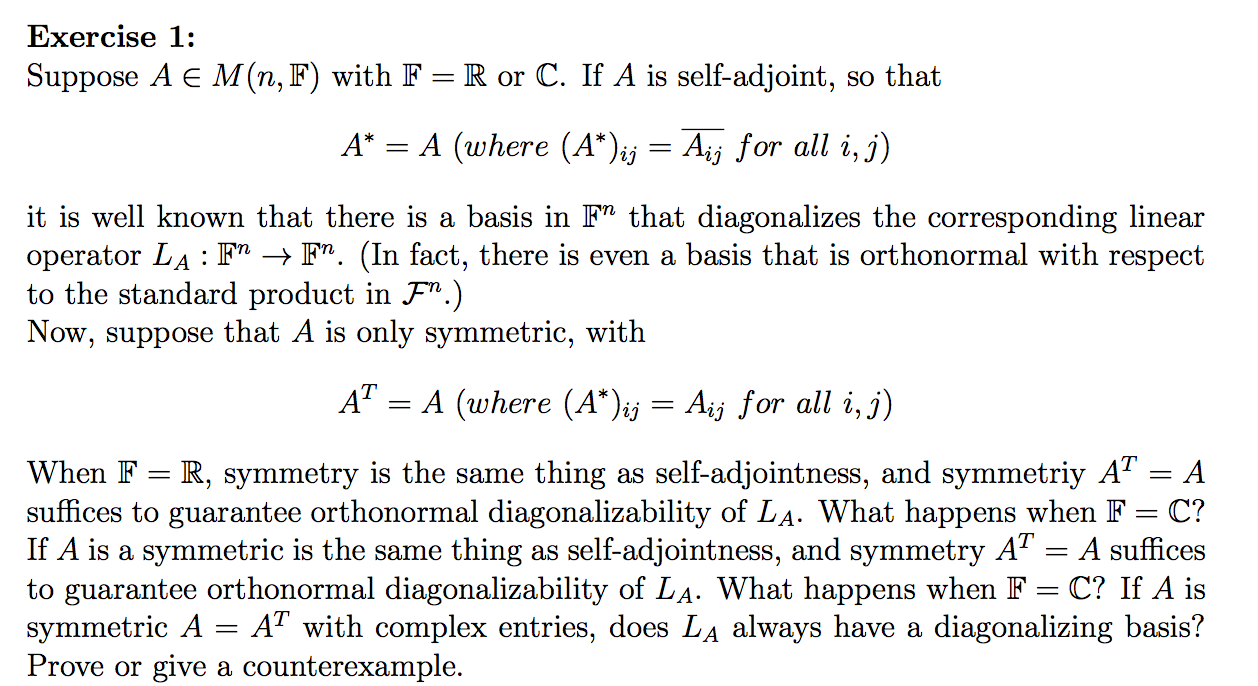
\includegraphics[width=1\textwidth]{LA-4-1.png}
\end{figure}
\end{question}
\begin{solution} \hfill \\
Consider the following matrix:
\eQb
\begin{pmatrix}
1 & i \\
i & -1 \\
\end{pmatrix}.
\eQe
The matrix equals its transpose, but not its conjugate transpose.
The characteristic polynomial of the matrix is $(1-\lambda)(-1-\lambda) + 1= \lambda^2$. Hence,
we obtain that the eigenvalue of the matrix is $0$ with algebraic multiplicity of $2$. Now, observe that 
$E_{\lambda=0}(L_A) = \text{Null}(L_A - 0I) = \text{Null}(L_A)$. 
Since the nullspace of $L_A$ is the span of row vectors of $A$, and
$(1,i)$ and $(i,-1)$ are linearly dependent (take $i$ and $-1$ as coefficients), 
we have that
the geometric multiplictiy of $0$ is $1$. Therefore, the eigenspaces of $L_A$ do not form
a direct sum of $\mathbb{C}^2$. Therefore, by the Spectral Theorem, 
the matrix is not diagonalizable. 
\hfill $\qed$

\end{solution}

\newpage

\begin{question}[2]
\hfill
\begin{figure}[h!]
  \centering
    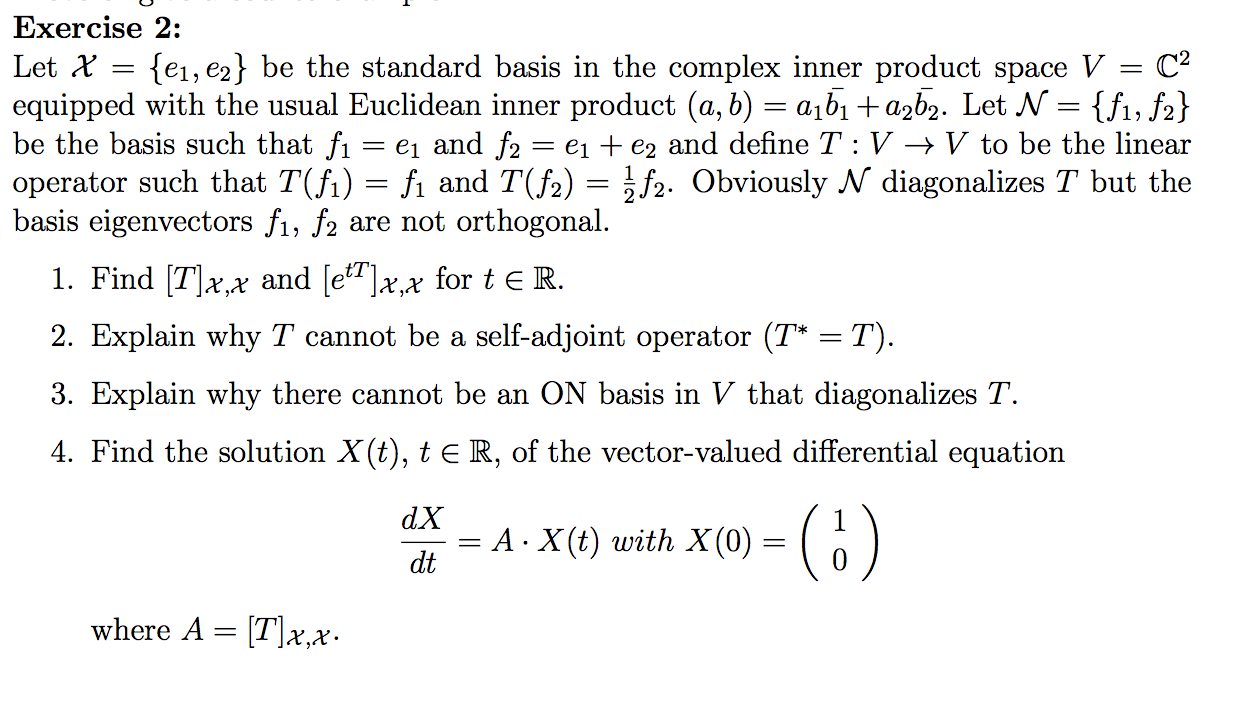
\includegraphics[width=1\textwidth]{LA-4-2.png}
\end{figure}
\end{question}
\begin{solution} \hfill \\
\textbf{(a)} 
With the given definition, we have
\eQb
T(e_1) &=& e_1, \\
T(e_2) &=& T(f_2 - e_1) = T(f_2) = T(e_1) = 
\dfrac{1}{2} f_2 + e_1 = -\dfrac{1}{2} e_1 + \dfrac{1}{2}e_2. 
\eQe
Therefore, it follows that
\eQb
[T]_{X,X} &=& \begin{pmatrix}
1 & \frac{-1}{2}  \\
0 & \frac{1}{2} \\
\end{pmatrix}.
\eQe

\bigskip

\textbf{(b)} 
We see that $T$ has a matrix representation with respect to the standard basis that is not
symmetric. Hence, $T^*$ cannot be self-adjoint.

\bigskip

\textbf{(c)}
Spectral theorem says that $T$ is orthonormally 
diagonalizable, iff $T$ is self-adjoint. Since $T$
is not self-adjoint, it is not orthonormally diagonalizable. 

\bigskip

\textbf{(d)}
The solution will be $[e^{tT}]$ where $t$ agrees with the initial data of $(1,0)$. 


\end{solution}

\newpage

\begin{question}[3]
\hfill
\begin{figure}[h!]
  \centering
    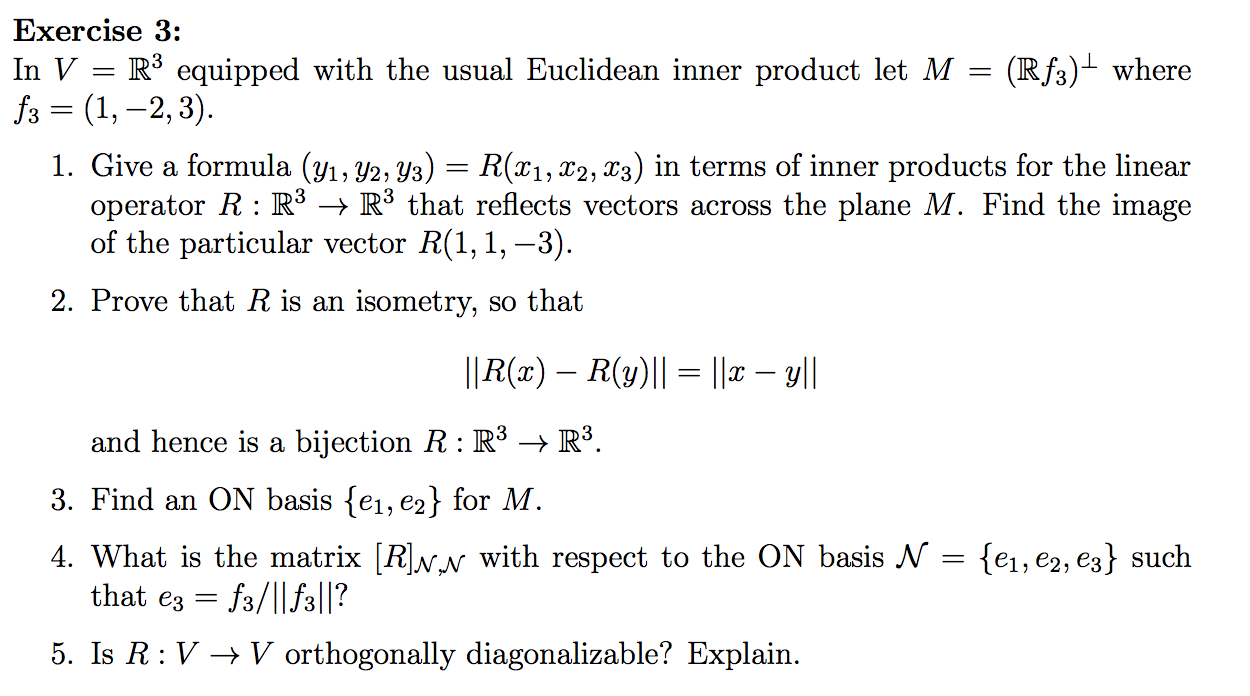
\includegraphics[width=1\textwidth]{LA-4-3.png}
\end{figure}
\end{question}
\begin{solution}
\textbf{(a)}
The reflection formula can be given by subtracting the orthogonal projection twice from
the original vector, which can be written as follows:
\eQb
R(v) &=& v - 2\dfrac{v \cdot f_3} {f_3 \cdot f_3}f_3.
\eQe

\smallskip

\textbf{(b)} From the above formula it follows that
\eQb
|| R(x) - R(y) || &=& ||x - 2\dfrac{x \cdot f_3}{f_3 \cdot f_3}f_3 - y + 2\dfrac{y \cdot f_3}
{f_3 \cdot f_3} f_3 || \\
&=& ||x -y - 2\dfrac{(x-y) \cdot f_3}{f_3 \cdot f_3} || \\
&=& || x- y||.
\eQe 

\smallskip

\textbf{(c)}
One can see that $(-1,1,1)$ has a $0$ inner product with $f_3$ and $(1,2,1)$ also have a $0$ inner
product and they are linearly independent. Therefore, they form an orthonormal basis for $M$.

\textbf{(e)}
We have that 

\hfill $\qed$

\end{solution}

\newpage

\begin{question}[4]
\hfill
\begin{figure}[h!]
  \centering
    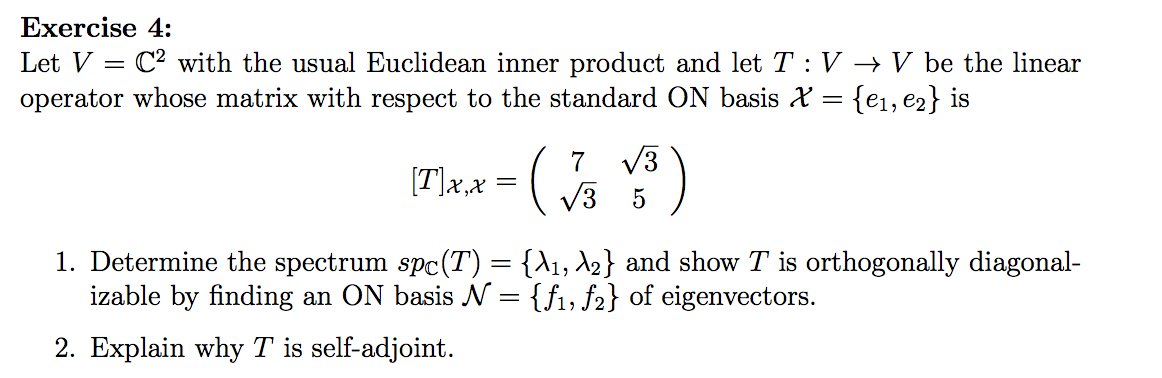
\includegraphics[width=1\textwidth]{LA-4-4.png}
\end{figure}
\end{question}
\begin{solution}
\textbf{(1)} The characteristic polynomial of $T$ can be computed as $(7 - \lambda)(5 - \lambda) -3
= \lambda^2 - 12\lambda + 32 = (\lambda - 8)(\lambda - 4)$. Therefore, we have that 
$\text{spec}_{\mathbb{C}}(T) = \{ 4, 8\}$. We see that the eigenvector associated with 
with $4$ is $\dfrac{1}{2}(1,-\sqrt{3})$ and with $8$ is $\dfrac{1}{2}(\sqrt{3},1)$, which 
are the $ON$ basis of eigenvectors, that orthogonally diagonalizes $T$. 

\smallskip

\textbf{(2)} When $T$ is a linear operator over complex field,
 that is represented in a matrix form with respect
to an orthonormal basis, we have that the matrix representation of $T^*$, with 
respect to the orthonormal basis, is the conjugate transpose
of the matrix representation of $T$. As operators with the same matrix representation
with respect to the same set of basis are in fact the same linear operator, we have that $T = T^*$,
which is the condition for a linear operator to be self-adjoint.

\hfill $\qed$ 
\end{solution}

\newpage

\begin{question}[4-continued]
\hfill
\begin{figure}[h!]
  \centering
    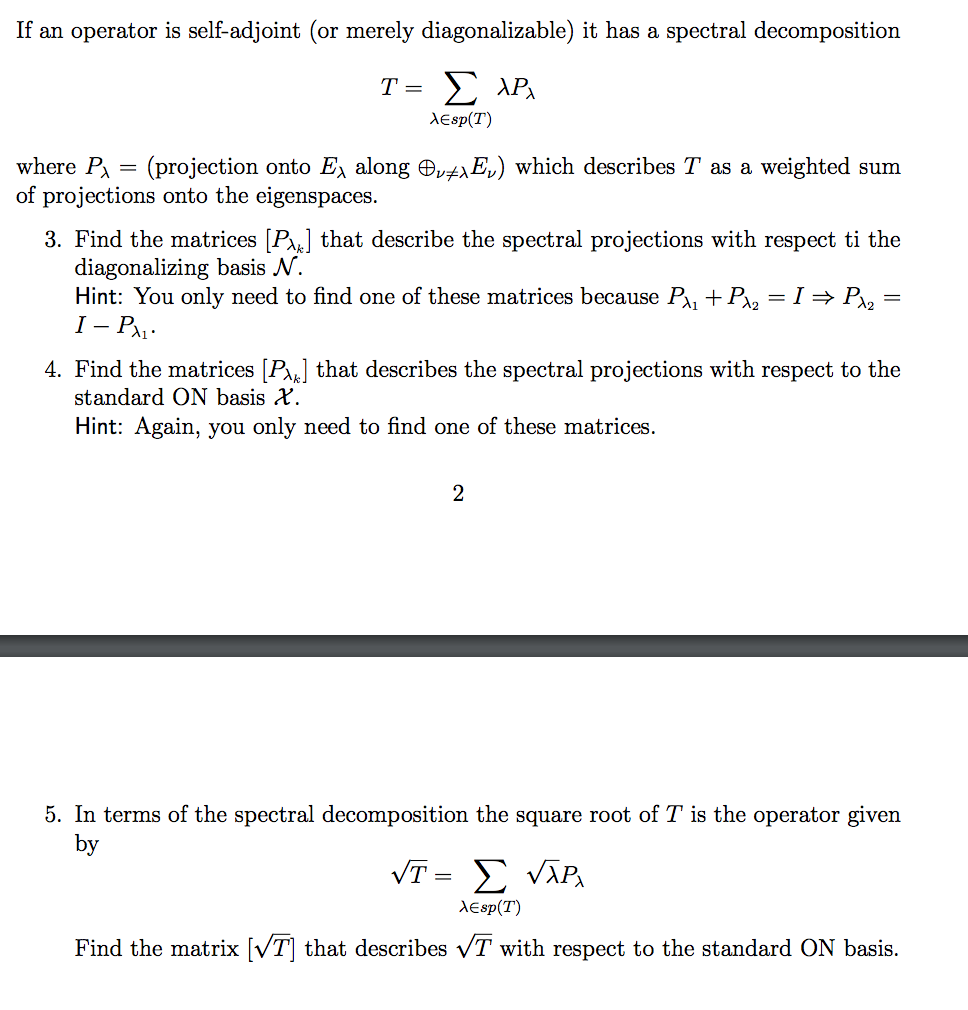
\includegraphics[width=1\textwidth]{LA-4-5.png}
\end{figure}
\end{question}
\begin{solution} \hfill \\
\textbf{(3)} By Spectral Theorem, we have
\eQb
P_{\lambda} &=& \prod_{u \neq \lambda} \dfrac{A - uI}{\lambda - u}.
\eQe
Hence, it follows that
\eQb
P_{\lambda = 8} &=& \dfrac{A - 4I}{8 - 4} \\
&=& \dfrac{1}{4} \begin{pmatrix}
3 & \sqrt{3} \\
\sqrt{3} & 1 \\
\end{pmatrix}  
\eQe


\hfill $\qed$ 

\end{solution}


\end{document}
